% Options for packages loaded elsewhere
\PassOptionsToPackage{unicode}{hyperref}
\PassOptionsToPackage{hyphens}{url}
%
\documentclass[
]{article}
\usepackage{lmodern}
\usepackage{amssymb,amsmath}
\usepackage{ifxetex,ifluatex}
\ifnum 0\ifxetex 1\fi\ifluatex 1\fi=0 % if pdftex
  \usepackage[T1]{fontenc}
  \usepackage[utf8]{inputenc}
  \usepackage{textcomp} % provide euro and other symbols
\else % if luatex or xetex
  \usepackage{unicode-math}
  \defaultfontfeatures{Scale=MatchLowercase}
  \defaultfontfeatures[\rmfamily]{Ligatures=TeX,Scale=1}
\fi
% Use upquote if available, for straight quotes in verbatim environments
\IfFileExists{upquote.sty}{\usepackage{upquote}}{}
\IfFileExists{microtype.sty}{% use microtype if available
  \usepackage[]{microtype}
  \UseMicrotypeSet[protrusion]{basicmath} % disable protrusion for tt fonts
}{}
\makeatletter
\@ifundefined{KOMAClassName}{% if non-KOMA class
  \IfFileExists{parskip.sty}{%
    \usepackage{parskip}
  }{% else
    \setlength{\parindent}{0pt}
    \setlength{\parskip}{6pt plus 2pt minus 1pt}}
}{% if KOMA class
  \KOMAoptions{parskip=half}}
\makeatother
\usepackage{xcolor}
\IfFileExists{xurl.sty}{\usepackage{xurl}}{} % add URL line breaks if available
\IfFileExists{bookmark.sty}{\usepackage{bookmark}}{\usepackage{hyperref}}
\hypersetup{
  pdftitle={Assignment 2 - Compiling Advanced R},
  pdfauthor={Chamundeswari Koppisetti},
  hidelinks,
  pdfcreator={LaTeX via pandoc}}
\urlstyle{same} % disable monospaced font for URLs
\usepackage[margin=1in]{geometry}
\usepackage{color}
\usepackage{fancyvrb}
\newcommand{\VerbBar}{|}
\newcommand{\VERB}{\Verb[commandchars=\\\{\}]}
\DefineVerbatimEnvironment{Highlighting}{Verbatim}{commandchars=\\\{\}}
% Add ',fontsize=\small' for more characters per line
\usepackage{framed}
\definecolor{shadecolor}{RGB}{248,248,248}
\newenvironment{Shaded}{\begin{snugshade}}{\end{snugshade}}
\newcommand{\AlertTok}[1]{\textcolor[rgb]{0.94,0.16,0.16}{#1}}
\newcommand{\AnnotationTok}[1]{\textcolor[rgb]{0.56,0.35,0.01}{\textbf{\textit{#1}}}}
\newcommand{\AttributeTok}[1]{\textcolor[rgb]{0.77,0.63,0.00}{#1}}
\newcommand{\BaseNTok}[1]{\textcolor[rgb]{0.00,0.00,0.81}{#1}}
\newcommand{\BuiltInTok}[1]{#1}
\newcommand{\CharTok}[1]{\textcolor[rgb]{0.31,0.60,0.02}{#1}}
\newcommand{\CommentTok}[1]{\textcolor[rgb]{0.56,0.35,0.01}{\textit{#1}}}
\newcommand{\CommentVarTok}[1]{\textcolor[rgb]{0.56,0.35,0.01}{\textbf{\textit{#1}}}}
\newcommand{\ConstantTok}[1]{\textcolor[rgb]{0.00,0.00,0.00}{#1}}
\newcommand{\ControlFlowTok}[1]{\textcolor[rgb]{0.13,0.29,0.53}{\textbf{#1}}}
\newcommand{\DataTypeTok}[1]{\textcolor[rgb]{0.13,0.29,0.53}{#1}}
\newcommand{\DecValTok}[1]{\textcolor[rgb]{0.00,0.00,0.81}{#1}}
\newcommand{\DocumentationTok}[1]{\textcolor[rgb]{0.56,0.35,0.01}{\textbf{\textit{#1}}}}
\newcommand{\ErrorTok}[1]{\textcolor[rgb]{0.64,0.00,0.00}{\textbf{#1}}}
\newcommand{\ExtensionTok}[1]{#1}
\newcommand{\FloatTok}[1]{\textcolor[rgb]{0.00,0.00,0.81}{#1}}
\newcommand{\FunctionTok}[1]{\textcolor[rgb]{0.00,0.00,0.00}{#1}}
\newcommand{\ImportTok}[1]{#1}
\newcommand{\InformationTok}[1]{\textcolor[rgb]{0.56,0.35,0.01}{\textbf{\textit{#1}}}}
\newcommand{\KeywordTok}[1]{\textcolor[rgb]{0.13,0.29,0.53}{\textbf{#1}}}
\newcommand{\NormalTok}[1]{#1}
\newcommand{\OperatorTok}[1]{\textcolor[rgb]{0.81,0.36,0.00}{\textbf{#1}}}
\newcommand{\OtherTok}[1]{\textcolor[rgb]{0.56,0.35,0.01}{#1}}
\newcommand{\PreprocessorTok}[1]{\textcolor[rgb]{0.56,0.35,0.01}{\textit{#1}}}
\newcommand{\RegionMarkerTok}[1]{#1}
\newcommand{\SpecialCharTok}[1]{\textcolor[rgb]{0.00,0.00,0.00}{#1}}
\newcommand{\SpecialStringTok}[1]{\textcolor[rgb]{0.31,0.60,0.02}{#1}}
\newcommand{\StringTok}[1]{\textcolor[rgb]{0.31,0.60,0.02}{#1}}
\newcommand{\VariableTok}[1]{\textcolor[rgb]{0.00,0.00,0.00}{#1}}
\newcommand{\VerbatimStringTok}[1]{\textcolor[rgb]{0.31,0.60,0.02}{#1}}
\newcommand{\WarningTok}[1]{\textcolor[rgb]{0.56,0.35,0.01}{\textbf{\textit{#1}}}}
\usepackage{graphicx,grffile}
\makeatletter
\def\maxwidth{\ifdim\Gin@nat@width>\linewidth\linewidth\else\Gin@nat@width\fi}
\def\maxheight{\ifdim\Gin@nat@height>\textheight\textheight\else\Gin@nat@height\fi}
\makeatother
% Scale images if necessary, so that they will not overflow the page
% margins by default, and it is still possible to overwrite the defaults
% using explicit options in \includegraphics[width, height, ...]{}
\setkeys{Gin}{width=\maxwidth,height=\maxheight,keepaspectratio}
% Set default figure placement to htbp
\makeatletter
\def\fps@figure{htbp}
\makeatother
\setlength{\emergencystretch}{3em} % prevent overfull lines
\providecommand{\tightlist}{%
  \setlength{\itemsep}{0pt}\setlength{\parskip}{0pt}}
\setcounter{secnumdepth}{-\maxdimen} % remove section numbering

\title{Assignment 2 - Compiling Advanced R}
\author{Chamundeswari Koppisetti}
\date{9/11/2020}

\begin{document}
\maketitle

\hypertarget{firtsly-have-set-the-current-working-directory}{%
\subsection{Firtsly, have set the current working
directory}\label{firtsly-have-set-the-current-working-directory}}

\begin{Shaded}
\begin{Highlighting}[]
\KeywordTok{setwd}\NormalTok{(}\StringTok{"D:/Courses/Stat 5361 - Statistical Computing/Assignment 2/adv-r"}\NormalTok{)}
\end{Highlighting}
\end{Shaded}

\hypertarget{upgraded-rstudio-from-older-version-to-4.0.2-and-installed-packages-to-the-latest-version}{%
\subsection{Upgraded RStudio from older version to 4.0.2 and installed
packages to the latest
version}\label{upgraded-rstudio-from-older-version-to-4.0.2-and-installed-packages-to-the-latest-version}}

\begin{Shaded}
\begin{Highlighting}[]
\CommentTok{# install.packages("installr")}
\CommentTok{# installr::updateR()}
\NormalTok{R.version}
\end{Highlighting}
\end{Shaded}

\begin{verbatim}
##                _                           
## platform       x86_64-w64-mingw32          
## arch           x86_64                      
## os             mingw32                     
## system         x86_64, mingw32             
## status                                     
## major          4                           
## minor          0.2                         
## year           2020                        
## month          06                          
## day            22                          
## svn rev        78730                       
## language       R                           
## version.string R version 4.0.2 (2020-06-22)
## nickname       Taking Off Again
\end{verbatim}

\hypertarget{steps-to-build-the-book-using-rstudio}{%
\subsection{Steps to build the book using
Rstudio}\label{steps-to-build-the-book-using-rstudio}}

\hypertarget{downloaded-the-sourcefile-from-compile-hadleys-advanced-r-to-a-pdf-httpsbrettklamer.comdiversionsstatisticalcompile-hadleys-advanced-r-programming-to-a-pdf}{%
\subsection{\texorpdfstring{1. Downloaded the sourcefile from
{[}\emph{Compile Hadley's Advanced R to a PDF}{]}
``\url{https://brettklamer.com/diversions/statistical/compile-hadleys-advanced-r-programming-to-a-pdf/}''}{1. Downloaded the sourcefile from {[}Compile Hadley's Advanced R to a PDF{]} ``https://brettklamer.com/diversions/statistical/compile-hadleys-advanced-r-programming-to-a-pdf/''}}\label{downloaded-the-sourcefile-from-compile-hadleys-advanced-r-to-a-pdf-httpsbrettklamer.comdiversionsstatisticalcompile-hadleys-advanced-r-programming-to-a-pdf}}

\hypertarget{installed-r-package-dependencies}{%
\subsection{2. Installed R Package
Dependencies:}\label{installed-r-package-dependencies}}

\begin{Shaded}
\begin{Highlighting}[]
\CommentTok{# install.packages('bookdown') }
\CommentTok{# install.packages("devtools")}

\CommentTok{# devtools::install_github("hadley/sloop")}
\CommentTok{# devtools::install_github("hadley/emo")}
\end{Highlighting}
\end{Shaded}

\hypertarget{used-the-below-to-compile-the-book}{%
\subsection{3. Used the below to compile the
book:}\label{used-the-below-to-compile-the-book}}

\begin{Shaded}
\begin{Highlighting}[]
\CommentTok{# bookdown::render_book("index.Rmd", output_format = "bookdown::pdf_book")}
\end{Highlighting}
\end{Shaded}

\hypertarget{below-are-the-error-messages-i-received-and-how-i-have-solved-them-during-the-building-process}{%
\subsection{Below are the error messages I received and how I have
solved them, during the building
process}\label{below-are-the-error-messages-i-received-and-how-i-have-solved-them-during-the-building-process}}

\begin{enumerate}
\def\labelenumi{\arabic{enumi}.}
\item
  Missing packages: Used `install.packages()' to install all these
  mentioned: \emph{lobstr}, \emph{ggplot2}, \emph{dplyr}, \emph{DBI},
  \emph{RSQLite}, \emph{zeallot}, \emph{dbplyr}, \emph{profvis},
  \emph{bench}, \emph{tidyr}, \emph{ggbeeswarm}
\item
  `make' not found: Installed \emph{Rtools} manually and added the path
  (`C:\rtools40\usr\bin') to Evironment variables
\end{enumerate}

\begin{Shaded}
\begin{Highlighting}[]
\NormalTok{knitr}\OperatorTok{::}\KeywordTok{include_graphics}\NormalTok{(}\StringTok{"D:/Courses/Stat 5361 - Statistical Computing/Assignment 2/Make.JPG"}\NormalTok{)}
\end{Highlighting}
\end{Shaded}

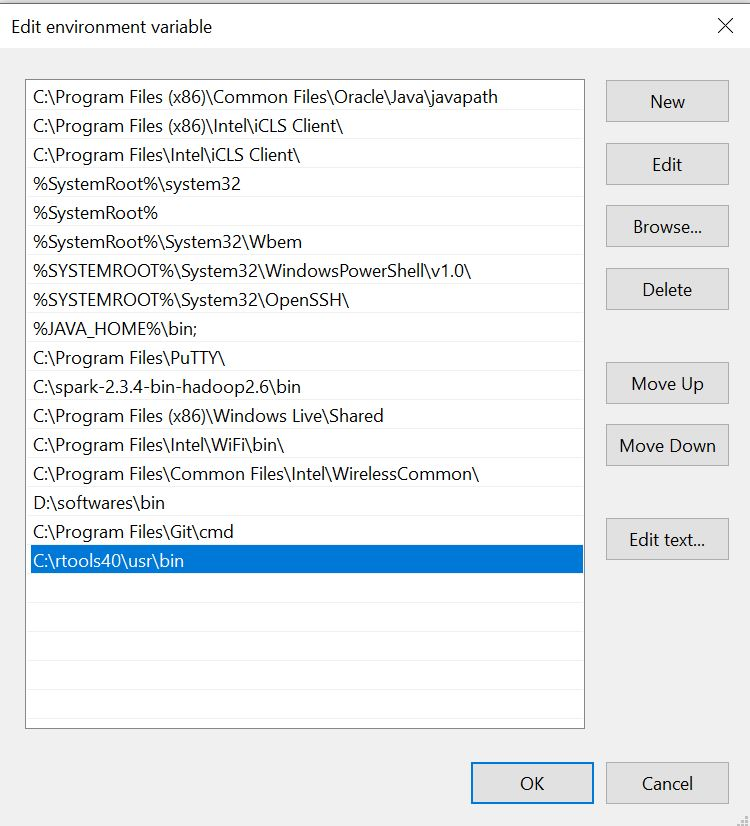
\includegraphics{D:/Courses/Stat 5361 - Statistical Computing/Assignment 2/Make.JPG}

\begin{Shaded}
\begin{Highlighting}[]
\CommentTok{## Cross checked the path name of 'make' after installation}

\KeywordTok{Sys.which}\NormalTok{(}\StringTok{'make'}\NormalTok{)}
\end{Highlighting}
\end{Shaded}

\begin{verbatim}
##                               make 
## "C:\\rtools40\\usr\\bin\\make.exe"
\end{verbatim}

\hypertarget{font-inconsolata-and-andalemono-not-found}{%
\subsection{3. Font ``Inconsolata'' and ``AndaleMono'' not
found:}\label{font-inconsolata-and-andalemono-not-found}}

3.1. Installed ``Tex Liv'' as it's much more stable to ``tinytex'' 3.2.
Downloaded `.ttf' and `.otf' files for ``Inconsolata'', and `.ttf' file
for ``AndaleMono'' 3.3. Saved Opentype file(.otf) into latex folder:
``C:/texlive/2020/texmf-dist/fonts/opentype/public/inconsolata'' True
typefile(.ttf) into latex folder:
``C:/texlive/2020/texmf-dist/fonts/truetype/public/inconsolata'',
``C:/texlive/2020/texmf-dist/fonts/truetype/public/andalemono''

\hypertarget{final-_main.pdf-is-generated}{%
\section{Final '\_main.pdf' is
generated}\label{final-_main.pdf-is-generated}}

\end{document}
